\documentclass[11pt]{article}

\author{wilricknl}
\title{3D Math Primer - Notes}

\usepackage{amsmath}
\usepackage{float}
\usepackage{tikz}
\usetikzlibrary{arrows.meta}

\begin{document}

\maketitle

\section{Introduction}

This document is a reference of the things most interesting to me from 3D math primer.

\section{Chapter 1}

\subsection{Coordinate system handedness}

In 3D space there are two types of coordinate systems: the so-called left and right handed coordinate systems. The way to recreate these systems is to make your index fingers pointer up, then your thumbs should point to each other, while your third finger points away from you. Just like in algebra class your index finger represents the $y$ axis, your thumbs the $x$ axis, while your third finger represents the $z$ axis.

\begin{figure}[H]
\centering
    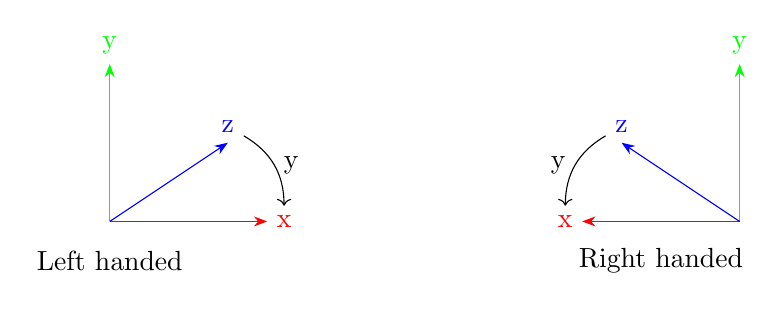
\begin{tikzpicture}
		\draw [red,-{Stealth}] (-4,0)--(-2,0) node[right] (xleft) {x};        
		\draw [green,-{Stealth}] (-4,0)--(-4,2) node[above]{y};       
		\draw [blue,-{Stealth}] (-4,0)--(-2.5,1) node[above] (zleft) {z};  
		\draw[->] (zleft) to[bend left] node [right] {y} (xleft);
		\node at (-4,-0.5) {Left handed};      
        
		\draw [red,{Stealth}-] (2,0) node[left] (xright) {x} -- (4,0);        
		\draw [green,-{Stealth}] (4,0)--(4,2) node[above]{y};       
		\draw [blue,-{Stealth}] (4,0)--(2.5,1) node[above] (zright) {z};
		\draw[->] (zright) to[bend right] node [left] {y} (xright);  
		\node at (3,-0.5) {Right handed};
		                
    \end{tikzpicture}
\caption{Coordinate system handedness}
\label{fig:coordinate-system-handedness}
\end{figure}

Rotation in a left handed in a left handed system is clock wise, while positive in a right handed system is counter clock wise. In figure  \ref{fig:coordinate-system-handedness} the $y$-rotation of both  coordinate systems is visualized with the black arrow. A trick to remember is to put your thumb up and see how your fingers curl around your palm.

\begin{quote}
\emph{Within these notes I follow the book and use the left handed system as visualized in figure \ref{fig:coordinate-system-handedness}.}
\end{quote}

\subsection{Trigonometry}

\subsubsection{Functions}

\begin{align*}
\cos\theta &=x, &\sin\theta &=y, \\
\sec\theta &=\frac{1}{\cos\theta}, &\tan\theta &=\frac{\sin\theta}{\cos\theta}, \\
\csc\theta &=\frac{1}{\sin\theta}, &\cot\theta &=\frac{1}{\tan\theta}=\frac{\cos\theta}{\sin\theta}.
\end{align*}

\subsubsection{Function definitions}

The primary function are defined by the ratios of a \emph{right} triangle. Note that when the angle is obtuse, i.e. $90^\circ < \theta < 180^\circ$, the ratios do not work.

% todo: angle diagram and functions
% todo: explain obtuse situation

\subsubsection{Identities}

\subsubsection{Common values}

% todo: the table with all those values. yup a pain

\subsubsection{Sum and difference identities}

% todo: identities

\subsubsection{Pythagorean identities}

% todo: identities + briefly mention pythagoras theorem

\subsubsection{Double angle identities}

% todo: identities

\subsubsection{Law of sines}

% todo: draw triangle to display these laws

$$\frac{\sin A}{a}=\frac{\sin B}{b}=\frac{\sin C}{c}$$

\subsubsection{Law of cosines}

% todo: reference triangle

\begin{align*}
a^2 &= b^2 + c^2 - 2bc\cos A, \\
b^2 &= a^2 + c^2 - 2ac\cos B, \\
c^2 &= a^2 + b^2 - 2ab\cos C.
\end{align*}

\end{document}
